\subsection{{\cjkfont 相同参数下的暗态正向检验}\allowbreak{}}
{\cjkfont 为检验上述反偏条件模型能否同时给出合理的另一极性响应，我们保持全部材料与接触参数不变，补算}\allowbreak{} 300{\cjkfont 、}\allowbreak{}340{\cjkfont 、}\allowbreak{}380{\cjkfont 、}\allowbreak{}420 K {\cjkfont 和两种接触情景的暗态正向曲线。电压从}\allowbreak{} 0 {\cjkfont 到}\allowbreak{} $+1.2$ V{\cjkfont ，步长}\allowbreak{} 0.05 V{\cjkfont ，共}\allowbreak{} 200 {\cjkfont 个稳态（含}\allowbreak{} 8 {\cjkfont 个平衡态）。正电压降低平衡内建电势落差；零偏净流为零，正向电流与正的端口耗散一致。没有为正偏或单个温度重新拟合参数。}\allowbreak{}

\textbf{{\cjkfont 高电流支路的限制。}\allowbreak{}}{\cjkfont 模型没有串联电阻、有限接触供给或热方程，并强制薄膜保持外加温度。精化后的}\allowbreak{} $b=0.4$ eV{\cjkfont 、}\allowbreak{}420 K{\cjkfont 、}\allowbreak{}$+1.2$ V {\cjkfont 给出约}\allowbreak{} $1175.53\,\mathrm{A\,cm^{-2}}${\cjkfont ，对应}\allowbreak{} $1410.64\,\mathrm{W\,cm^{-2}}${\cjkfont 。这一结果暴露了理想边界与等温近似的现实限制，不能解释为真实器件可维持的工作状态。数值收敛不等于物理预测可信。}\allowbreak{}

\begin{figure}[htbp]\centering
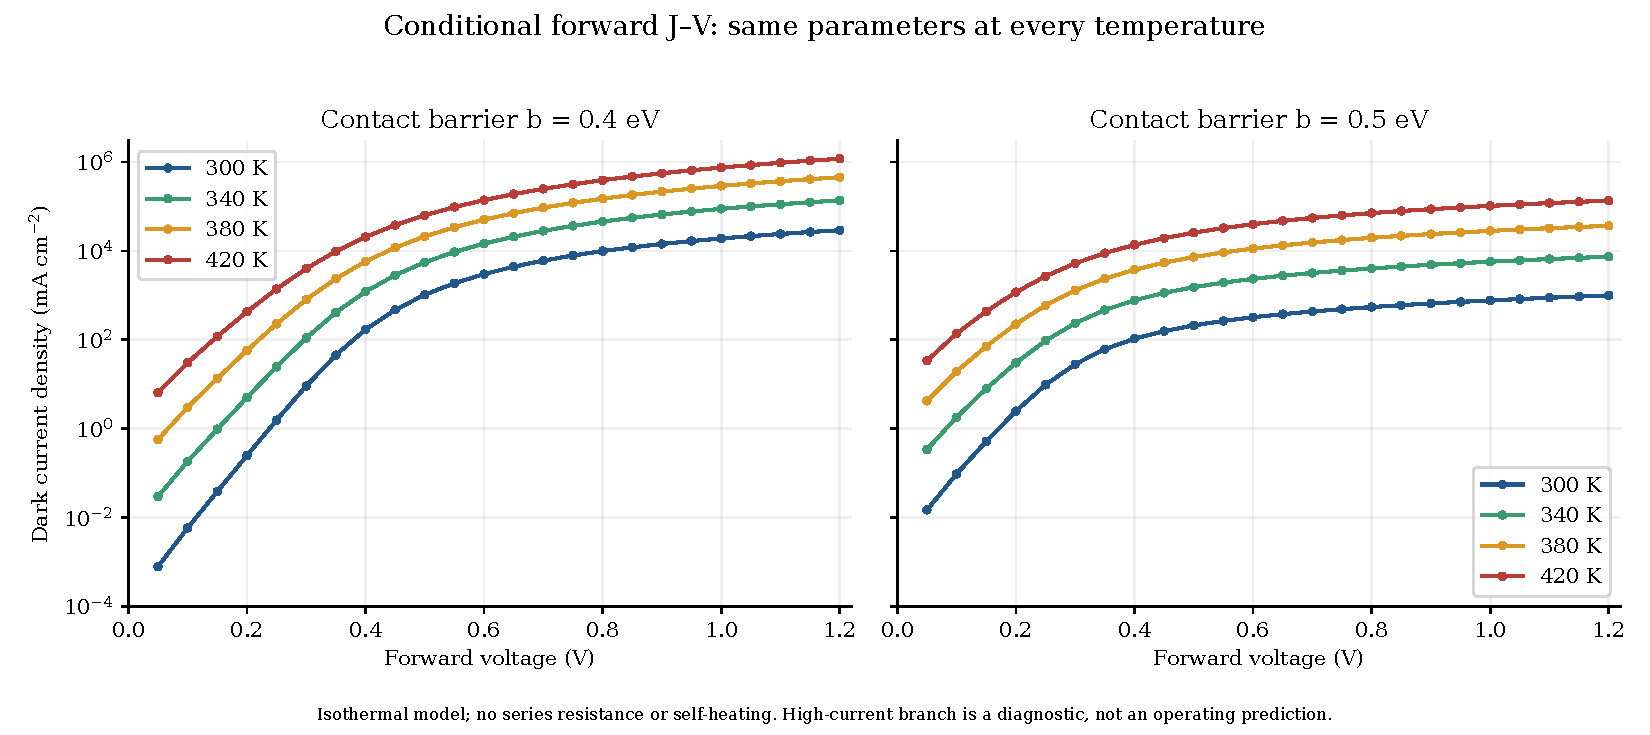
\includegraphics[width=.98\linewidth]{figures/forward_temperature_JV.pdf}
\caption{{\cjkfont 相同参数下的八条暗态正向温度曲线，主图采用}\allowbreak{} 161 {\cjkfont 节点。高正偏部分为无串联电阻和无自热反馈的理想方程诊断，不能当作真实工作电流。这里没有光照，不能计算太阳能电池的}\allowbreak{} FF {\cjkfont 或效率。}\allowbreak{}}
\end{figure}

\begin{table}[htbp]\centering\small
\begin{tabular}{rrrrrr}\toprule
$b$ (eV)&$V$ (V)&300 K&340 K&380 K&420 K\\\midrule
0.4&$+0.1$&$5.879\times10^{-6}$&$1.842\times10^{-4}$&0.003028&0.03059\\
0.4&$+0.3$&0.009136&0.1102&0.8034&3.984\\
0.4&$+0.5$&1.030&5.545&21.12&63.08\\
0.5&$+0.1$&$9.624\times10^{-5}$&0.001818&0.01948&0.1385\\
0.5&$+0.3$&0.02829&0.2365&1.298&5.241\\
0.5&$+0.5$&0.2109&1.527&7.275&25.65\\\bottomrule
\end{tabular}
\caption{{\cjkfont 暗态正向代表点的}\allowbreak{} $J${\cjkfont ，单位}\allowbreak{} $\mathrm{A\,cm^{-2}}${\cjkfont 。与前文反偏表的毫安单位不同；这些数值属于条件模型，尚无同样品变温正向数据逐点验证。}\allowbreak{}}
\end{table}

{\cjkfont 在}\allowbreak{} $b=0.4$ eV {\cjkfont 情景，}\allowbreak{}420/300 K {\cjkfont 电流比从}\allowbreak{} $+0.1$ V {\cjkfont 的约}\allowbreak{} 5203 {\cjkfont 变为}\allowbreak{} $+0.3$ V {\cjkfont 的}\allowbreak{} 436{\cjkfont 、}\allowbreak{}$+1.0$ V {\cjkfont 的}\allowbreak{} 39.3{\cjkfont ；四温度表观激活能相应约为}\allowbreak{} 0.774{\cjkfont 、}\allowbreak{}0.550{\cjkfont 、}\allowbreak{}0.332 eV{\cjkfont 。这种电压依赖包含输运、接触供给、空间电荷和复合的共同变化，不能直接读成一个陷阱深度。}\allowbreak{}

200 {\cjkfont 点通过电流、电荷、能量与四速率详细平衡检查。四个代表工况进一步作}\allowbreak{} 161{\cjkfont 、}\allowbreak{}321{\cjkfont 、}\allowbreak{}641 {\cjkfont 节点比较，后两者电流最大变化}\allowbreak{} 0.134\%{\cjkfont ，}\allowbreak{}161 {\cjkfont 到}\allowbreak{} 641 {\cjkfont 最大变化}\allowbreak{} 0.519\%{\cjkfont ；并非全部}\allowbreak{} 200 {\cjkfont 点都做过三网格检验。两代表点将高斯积分从}\allowbreak{} 128 {\cjkfont 增至}\allowbreak{} 256 {\cjkfont 阶，端电流变化分别为}\allowbreak{} $3.83\times10^{-10}$ {\cjkfont 和}\allowbreak{} $1.21\times10^{-11}${\cjkfont 。最高节点占据约}\allowbreak{} $6.14\times10^{-4}${\cjkfont ，最大约化场}\allowbreak{} $qFa/\sigma=0.151${\cjkfont ，没有高占据或高场外推。}\allowbreak{}

{\cjkfont 正向曲线构成相同条件参数的额外一致性检验，尚没有配套的同材料、同温度暗态正向文献数据进入比较。结合反偏}\allowbreak{} S10 {\cjkfont 的温度差距，它要求今后同时约束接触、无序、迁移率和串联电阻；不能只调一个电阻降低正向电流而忽略反偏。这里不报告光照}\allowbreak{} $V_{\rm oc}${\cjkfont 、}\allowbreak{}$J_{\rm sc}${\cjkfont 、}\allowbreak{}FF {\cjkfont 或效率，也不沿用旧}\allowbreak{} FF78 {\cjkfont 值。}\allowbreak{}

